\chapter{Análise dos resultados}
\label{cap:resultados}

As métricas coletadas foram analisadas com base no levantamento teórico realizado, buscando avaliar os aspectos de desempenho de maneira objetiva e fundamentada em cada cenário analisado. Os valores apresentados neste capítulo correspondem à média dos resultados obtidos nos três computadores descritos na metodologia.

Para o tempo de execução, foi comparado o resultado entre os dois ambientes, expressando a diferença como \emph{overhead} percentual e fator multiplicativo.

Para o consumo de memória, foram aplicadas as métricas de \emph{baseline}, pico e consumo líquido descritas anteriormente, a fim de isolar o consumo efetivo do algoritmo do \emph{overhead} fixo do ambiente de execução Wasm.

A utilização de CPU, embora coletada, não é apresentada como resultado, pois foi empregada apenas para identificar os períodos de execução, pelos motivos descritos na Seção~\ref{sec:consumo-memoria}.

\section{Tempo de Execução}

A Tabela~\ref{tab:tempo} apresenta os tempos médios de execução obtidos nos ambientes Rust e WebAssembly para os cinco algoritmos avaliados, além do \emph{overhead} percentual e do fator multiplicativo, calculados pelas Equações~\eqref{eq:overhead} e~\eqref{eq:fator} a partir das médias dos três computadores (Equação~\eqref{eq:media-computadores}). Os resultados mostram que o \emph{overhead} variou de 10,9\% a 126,9\%, indicando diferenças distintas entre os algoritmos avaliados. Em todos os casos, o WebAssembly apresentou tempo de execução maior que o Rust nativo.
\begin{table}[H]
    \caption{ Comparativo de tempo de execução médio (ms) }
    \label{tab:tempo}
    \centering
    \setlength{\tabcolsep}{5pt}
    \begin{tabular}{ccccccc}
        \hline
        Algoritmo &Rust (ms) &Wasm (ms) &Overhead (\%) &Fator \\
        \hline
        fannkuch-redux &21.226,7 &23.539,7 &10,9 &1,109x \\
        \hline
        spectral-norm &1.271,7 &1.436,2 &12,9 &1,129x \\
        \hline
        fasta &1.701,5 &2.061,5 &21,2 &1,212x \\
        \hline
        n-body &1.907,7 &3.227,3 &69,2 &1,692x \\
        \hline
        mandelbrot &3.253,5 &7.381,7 &126,9 &2,269x \\
        \hline
    \end{tabular}
    \fonte{Os autores}
\end{table}

Os menores \emph{overheads} foram observados em fannkuch-redux e spectral-norm, com 10,9\% e 12,9\%, respectivamente. Em contraste, n-body e mandelbrot apresentaram as maiores diferenças, com 69,2\% e 126,9\%. A Figura~\ref{fig:grafico-tempo-benchmarking} permite visualizar essas diferenças entre os tempos médios de execução nos dois ambientes.

\begin{figure}[!htb]
	\centering
	\caption{Comparativo de tempo de execução médio}
    \label{fig:grafico-tempo-benchmarking}
	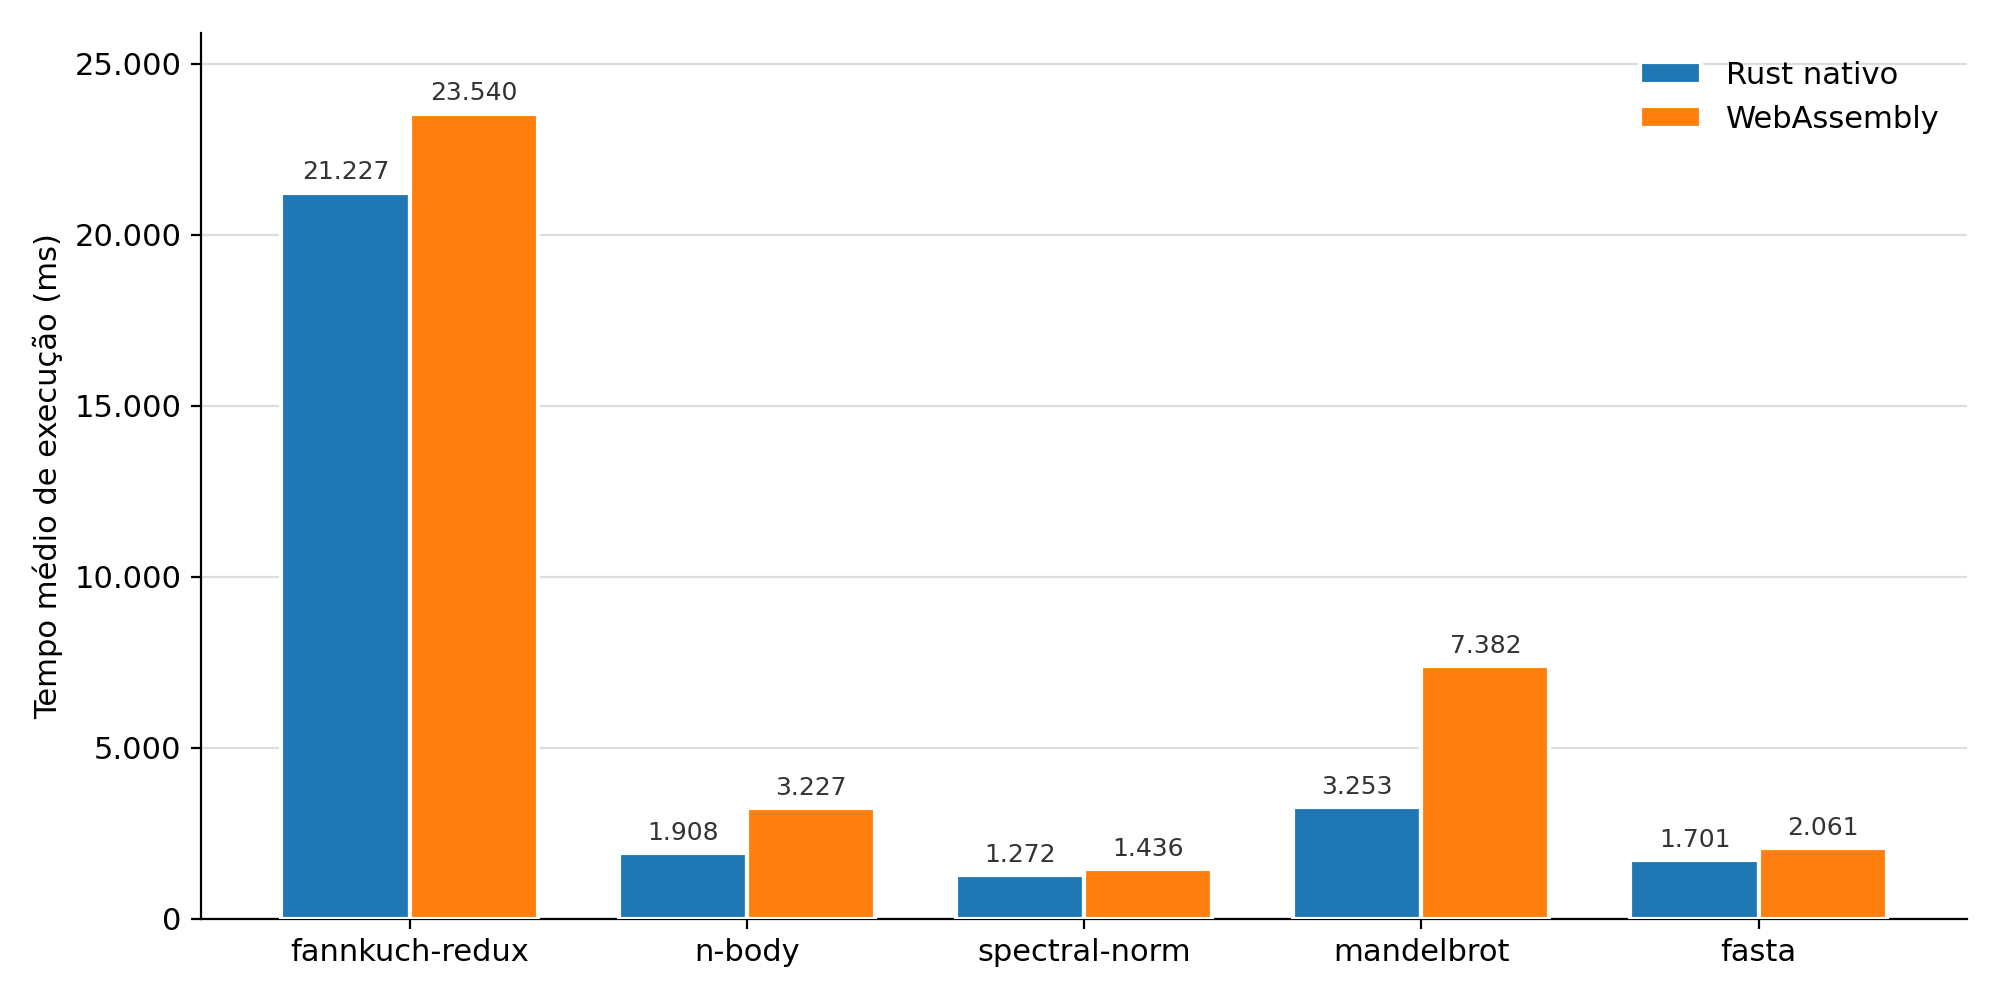
\includegraphics[width=\textwidth]{media/grafico-tempo-benchmarking}
    \fonte{Os autores}
\end{figure}

O algoritmo fannkuch-redux registrou o menor \emph{overhead}, correspondente a 10,9\%, ou fator 1,109x. Trata-se de um algoritmo baseado em permutações de vetores de inteiros de tamanho fixo, com operações predominantemente inteiras.

O spectral-norm apresentou \emph{overhead} de 12,9\%. O algoritmo realiza operações de ponto flutuante de dupla precisão em laços sobre vetores.

O algoritmo fasta obteve \emph{overhead} de 21,2\%. Sua execução envolve a geração de números pseudoaleatórios, consultas a tabelas de probabilidade acumulada e a escrita das sequências geradas em blocos de memória.

O n-body registrou \emph{overhead} de 69,2\%. A simulação envolve cálculos iterativos de forças gravitacionais entre cinco corpos, com uso intensivo de operações de ponto flutuante de dupla precisão, incluindo raízes quadradas, sobre um conjunto reduzido de dados.

O mandelbrot apresentou o maior \emph{overhead} observado, correspondente a 126,9\%. Nesse cenário, o tempo de execução em WebAssembly foi mais que o dobro do observado na execução nativa. O algoritmo realiza processamento intensivo de ponto flutuante de dupla precisão e grava o resultado em um \emph{buffer} de \emph{bits}.

Considerando todos os algoritmos avaliados, o \emph{overhead} médio foi de 48,2\% (Equação~\eqref{eq:media-overhead}), enquanto a mediana foi de 21,2\% (Equação~\eqref{eq:mediana-overhead}). A diferença entre essas métricas indica que os casos extremos, especialmente o mandelbrot, exercem influência significativa sobre a média geral dos resultados.

Os valores absolutos de tempo variaram entre os três computadores, que possuem configurações de \emph{hardware} e sistema operacional distintas, e o \emph{overhead} de alguns algoritmos também oscilou entre as máquinas, como no fannkuch-redux, entre 4,0\% e 18,0\%, e no spectral-norm, entre 7,6\% e 26,6\%. Ainda assim, a separação entre os grupos se manteve em todas elas: mandelbrot e n-body registraram os maiores \emph{overheads} nos três computadores, enquanto fannkuch-redux, spectral-norm e fasta permaneceram abaixo de 27\%.

\section{Uso de Memória}

As métricas de \emph{baseline}, pico e consumo líquido foram calculadas pelas Equações~\eqref{eq:baseline} a~\eqref{eq:liquido} para cada computador e consolidadas pela média entre eles (Equação~\eqref{eq:media-computadores}). As Tabelas~\ref{tab:memoria-rust} e~\ref{tab:memoria-wasm} apresentam os resultados obtidos.

\begin{table}[!h]
    \caption{Consumo de memória do executável Rust (MiB)}
    \label{tab:memoria-rust}
    \centering
    \setlength{\tabcolsep}{6pt}
    \begin{tabular}{lccc}
        \hline
        Algoritmo & Base & Pico & Líquido \\
        \hline
        fannkuch-redux  & 16,6 & 17,7 & 1,1 \\
        n-body          & 7,9  & 8,6  & 0,7 \\
        spectral-norm   & 8,1  & 9,0  & 1,0 \\
        mandelbrot      & 8,0  & 40,4 & 32,3 \\
        fasta           & 7,9  & 9,1  & 1,2 \\
        \hline
    \end{tabular}
    \fonte{Os autores}
\end{table}

\begin{table}[!h]
    \caption{Consumo de memória do executável WebAssembly (MiB)}
    \label{tab:memoria-wasm}
    \centering
    \setlength{\tabcolsep}{6pt}
    \begin{tabular}{lccc}
        \hline
        Algoritmo & Base & Pico & Líquido \\
        \hline
        fannkuch-redux  & 218,6 & 237,0 & 18,4 \\
        n-body          & 209,9 & 213,7 & 3,8 \\
        spectral-norm   & 209,6 & 211,7 & 2,2 \\
        mandelbrot      & 209,9 & 245,9 & 36,1 \\
        fasta           & 209,9 & 212,7 & 2,8 \\
        \hline
    \end{tabular}
    \fonte{Os autores}
\end{table}

O \emph{baseline} do ambiente Rust situou-se entre 7,9 MiB e 16,6 MiB, refletindo principalmente o consumo do contêiner em estado ocioso. O valor mais alto, observado no fannkuch-redux, decorre de um dos computadores, que registrou 32,1 MiB nessa execução, enquanto os demais ficaram próximos de 9 MiB. No ambiente WebAssembly, os valores de \emph{baseline} variaram entre 209,6 MiB e 218,6 MiB, em razão da execução permanente do Chrome Headless e do Puppeteer.

Dessa forma, a comparação direta entre os valores totais de memória não é adequada para avaliar exclusivamente o impacto dos algoritmos. Por esse motivo, a análise foi concentrada no consumo líquido de memória.

Considerando essa métrica, o Rust apresentou consumo líquido entre 0,7 MiB e 1,2 MiB em quatro dos cinco algoritmos: fannkuch-redux, n-body, spectral-norm e fasta. A exceção foi o mandelbrot, com 32,3 MiB, valor praticamente idêntico nos três computadores e compatível com o \emph{buffer} de saída alocado pelo algoritmo, que armazena um \emph{bit} por \emph{pixel} de uma imagem de 16.000 por 16.000 \emph{pixels}, totalizando cerca de 30,5 MiB.

No WebAssembly, o consumo líquido ficou entre 2,2 MiB e 3,8 MiB para n-body, spectral-norm e fasta, ligeiramente acima dos valores do Rust nativo. O mandelbrot também apresentou o maior consumo nesse ambiente, com 36,1 MiB, valor igualmente compatível com o \emph{buffer} de saída, que no WebAssembly é alocado na memória linear do módulo. O fannkuch-redux registrou 18,4 MiB, porém com grande variação entre os computadores, de 4,2 MiB a 39,5 MiB.

De modo geral, o consumo líquido do WebAssembly foi maior que o do Rust nativo em todos os algoritmos.

\section{Síntese comparativa}

Os resultados mostram que o Rust nativo foi mais rápido em todos os algoritmos e que o \emph{overhead} do WebAssembly variou de forma expressiva conforme o algoritmo. Fannkuch-redux, spectral-norm e fasta ficaram entre 10,9\% e 21,2\%, enquanto n-body e mandelbrot chegaram a 69,2\% e 126,9\%, separação que se manteve nos três computadores.

Também o ambiente WebAssembly exige, em repouso, cerca de 200 MiB a mais que o ambiente nativo, com \emph{baseline} de cerca de 210 MiB, contra 7,9 MiB a 16,6 MiB no Rust, para manter o Chrome Headless através do Puppeteer em execução, valor praticamente constante entre os algoritmos e independente da carga processada, tornando a comparação direta com o ambiente nativo inadequada. Por esse motivo, a análise de consumo de memória foi concentrada no consumo líquido, que isolou o impacto do algoritmo em execução. Por essa métrica, os dois ambientes apresentaram consumo reduzido na maioria dos algoritmos, com o WebAssembly ligeiramente acima do Rust nativo, e o maior consumo em ambos foi o do mandelbrot, determinado pelo tamanho do \emph{buffer} de saída.

\section{Limitações do estudo}

Há limitações que devem ser consideradas neste estudo:

\begin{itemize}
    \item Nos testes realizados, a variável de ambiente \texttt{RAYON\_NUM\_THREADS} foi fixada em 1, restringindo a execução de algoritmos que utilizam a biblioteca \emph{Rayon} a uma única \emph{thread}, mesmo naqueles casos em que o processamento paralelo poderia representar ganhos de desempenho. Essa restrição foi necessária em razão de erros encontrados na compilação da biblioteca \emph{wasm-bindgen-rayon} para o ambiente WebAssembly, e foi replicada no ambiente Rust nativo para manter a padronização entre as comparações.
    \item Estudos futuros poderiam empregar ambientes de execução WebAssembly independentes de navegador, como \emph{Wasmer} e \emph{Wasmtime}, permitindo isolar de forma mais precisa o desempenho do código WebAssembly.
    \item A avaliação do ambiente WebAssembly limitou-se ao navegador Google Chrome, controlado por meio do Puppeteer, o que restringe a generalização dos resultados obtidos. Diferentes navegadores utilizam motores de execução WebAssembly distintos, cada um com estratégias próprias de otimização, o que pode alterar significativamente os resultados de desempenho.
\end{itemize}
